% It also requires running BibTeX. The commands are as follows:
%
%  1)  latex  aipsamp
%  2)  bibtex aipsamp
%  3)  latex  aipsamp
%  4)  latex  aipsamp
% Use the file aiptemplate.tex as a template for your document.
\documentclass[%
 aip,
%jmp,%
%bmf,%
%sd,%
rsi,%
 amsmath,amssymb,
%preprint,%
 reprint,%
%author-year,%
author-numerical,%
]{revtex4-1}

\usepackage{graphicx}% Include figure files
\usepackage{dcolumn}% Align table columns on decimal point
\usepackage{bm}% bold math
\usepackage{float}
%\usepackage[mathlines]{lineno}% Enable numbering of text and display math
%\linenumbers\relax % Commence numbering lines

\begin{document}

\preprint{AIP/123-QED}

\title[Physics 111B- Gamma Ray Spectroscopy (GMA) Lab]{Gamma Ray Spectroscopy}


\author{Brandon Tran}
 \email{brandontran7758@berkeley.edu.}
\author{Lab Partner: Lok Ching Lui}%
\affiliation{$^1$Department of Physics, University of California, Berkeley%\\This line break forced with \textbackslash\textbackslash
}%


\date{\today}

\begin{abstract}

In this experiment, the gamma ray spectra of four radioactive sources, i.e., $\mathrm { ^ { 60 }Co}  $, $\mathrm {  ^ { 137 }Cs }$, $\mathrm { ^ { 22 }Na }$, and $\mathrm { ^ { 54 }Mn } $ will be collected using a NaI scintillation detector, a photomultiplier tube (PMT), an external amplifier, and a pulse height analyzer (PHA). First, the capabilities of the equipment, including the linearity of the amplifier and the gain of the photomultiplier tube, will be determined to provide the best possible calibration settings to collect the gamma ray spectra. The spectras will be analyzed to determine the backscatter peaks, Compton edges, and photopeaks of each source.. By varying the source distance from the detector, the absolute intensity of $\mathrm {  ^ { 137 }Cs }$ and the inverse square law will also be determined.  Lastly, the mass attenuation coefficients of $\mathrm { Al}$, $\mathrm {Cu}$, and $\mathrm {Pb}$ will be calculated from the $\mathrm { ^ { 137 }Cs } $ and $\mathrm { ^ { 22 }Na }$ sources.

\end{abstract} 

\keywords{pulse height analyzer, radioactive decay, detection, gamma ray, scintillation}

\maketitle



\section{Introduction \& Theory: Interaction of Gamma Ray Radiation with Matter}
Gamma rays ($\gamma$) or gamma radiation are high energy electromagnetic radiation arising from the radioactive decay of atomic nuclei. They have the shortest wavelength out of all electromagnetic waves and therefore are the most energetic form of electromagnetic radiation. Because of this, gamma rays are a form of ionizing radiation and are biologically hazardous. Unlike alpha and beta radiation, their high penetration power can lead to biological damage and requires shielding using dense materials like lead. \newline
\indent The energy spectrum of gamma rays can be used to identify the decaying nuclides using spectroscopy through the gamma ray's interaction with matter. While many gamma ray-matter interaction mechanisms exists, the three most important processes for radiation measurement are the photoelectric effect, Compton scattering, and pair production.\cite{Knoll} 


\subsection{The Photoelectric Effect}
In the photoelectric effect, an incoming gamma ray photon is completely absorbed by an atom and thus liberates a photoelectron with an energy of 

\begin{equation}
E _ { e ^ { - } } = E_{\gamma} - E _ { b }
\label{eq:one}
\end{equation}

\noindent where $E_{\gamma}$ is the energy of the gamma ray and $E _ { b }$ is the binding energy of the electron. For gamma ray energies of more than a few hundred keV, the photoelectron carries away most of the incoming photon's original energy. This photoelectron corresponds to the photopeak in Fig.~\ref{fig:compton}.


\subsection{Compton Scattering}
Compton scattering is the most predominant process in the isotope sources that this experiment uses. In this process, an incoming gamma ray is deflected at an angle $\theta$ from its original direction. This gamma ray photon transfers only a portion of its energy to the electron of an absorbing material. Using conservation of momentum and energy, it can be shown that

\begin{equation}
E_{\gamma \prime} = \frac {E_{\gamma}} { 1 + \frac { E_{\gamma} } { m _ { 0 } c ^ { 2 } } ( 1 - \cos \theta ) }
\label{eq:two}
\end{equation}

\noindent where $m _ { 0 } c ^ { 2 }$ is the rest mass energy of the electron, $E_{\gamma \prime} $ is the scattered photon energy, and $E_{\gamma}$ is the incoming gamma ray photon energy. Thus the energy transferred to the electron is 

\begin{equation}
E _ { e ^ { - } } = E_{\gamma} - E_{\gamma \prime} = E_{\gamma}[ \frac { \frac { E_{\gamma}} { m _ { 0 } c ^ { 2 } } ( 1 - \cos \theta ) } { 1 + \frac { E_{\gamma}} { m _ { 0} c ^ { 2 }} ( 1 - \cos \theta ) } ]
\label{eq:three}
\end{equation}

It can also be seen that the maximum energy  ($\theta=\pi$)  that can be transferred to the electron through Compton scattering is 

\begin{equation}
 E _ { e ^ { - } } | _ { \theta = \pi } = \frac { E_{\gamma} } { 1 + \frac{ m _ { 0 } c ^ { 2 }} {2E_{\gamma} }} 
 \label{eq:four}
\end{equation}

This max energy corresponds to the "Compton edge" in Fig.~\ref{fig:compton}. Since photons can be scattered for angles from 0 to $\pi$, we also have rise to the "Compton plateau" or the "Compton continuum" as demonstrated in Fig.~\ref{fig:compton} also. 

\begin{figure*}
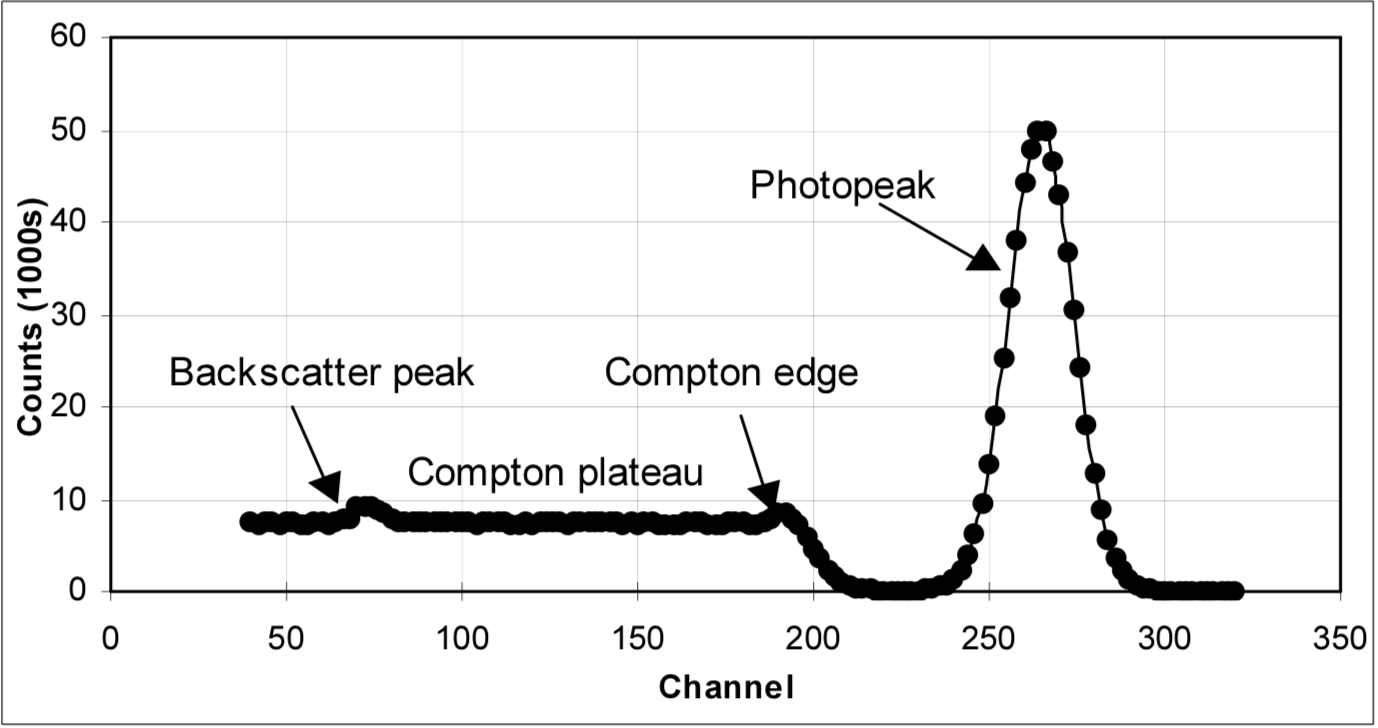
\includegraphics[width=0.6\linewidth]{lateximages/Spectra.png} 
\caption{\label{fig:compton}  Simplified version of a pulse height spectrum for a monochromatic gamma ray source. The Compton plateau arises when Compton scattering occurs in the detector, reaching a max energy ($\theta=\pi$) at the Compton edge. The backscatter peak is also a Compton event in which photons Compton scatter outside the detector before going into the detector. The photopeak corresponds to the photoelectric effect when the incoming gamma ray is completely absorbed by the detector material. (Source: Ref 2)}
\end{figure*}

Some gamma ray photons can also undergo one or more Compton scattering events by interacting with the surrounding material in the experiment before entering the detector material. This leads to what is known as the backscatter peak (Fig.~\ref{fig:compton}), which can be shown to have an energy of approximately

\begin{equation}
 E _ { back} = \frac { E_{\gamma} } { 1 + 4 E_{\gamma}} 
 \label{eq:five}
\end{equation}

\noindent or approximately the energy of the incoming gamma ray photon minus the Compton edge energy.


\subsection{Pair production}
Lastly, pair production is energetically possible if the incoming gamma ray is more than twice the rest mass energy of the electron (1.022 MeV). In this process, the gamma ray photon disappears and creates an electron-positron pair. The energy of the gamma ray in excess of 1.022 MeV becomes the kinetic energy of the electron and positron. This kinetic energy is quickly absorbed in the detector and can annihilate with an electron producing two 0.511 MeV gamma rays. \cite{florida} If both annihilation gammas are absorbed, the total energy absorbed will be the original gamma energy and the event would contribute to the photopeak. However, sometimes either or both of the annihilation gammas will escape from the crystal producing small peaks which are called single or double escape peaks that are 0.511 MeV or 1.022 MeV below the photopeak.

\section{Radioactive Decay Process of $^ {\textbf{60}}\textbf{Co}$, $^ {\textbf{137}}\textbf{Cs}$, $^ {\textbf{22}}\textbf{Na}$, and $^ {\textbf{54}}\textbf{Mn}$ }
The radioactive sources used in this experiment are $\mathrm { ^ { 60 }Co}  $, $\mathrm {  ^ { 137 }Cs }$, $\mathrm { ^ { 22 }Na }$, and $\mathrm { ^ { 54 }Mn } $. The processes by which they decay to produce gamma rays are discussed in the following section.

\subsection{Cobalt 60 Decay Process}
Cobalt decays to various forms of excited Nickel through beta decay. The end result are gamma ray energies of 1.173 MeV and 1.332 MeV. The following net reaction occurs approximately 99\% of the time.
\[\begin{array}{c} { _{27}^ { 60 }\mathrm { Co }  \rightarrow _{28} ^ { 60 }\mathrm { Ni } ^ { * } + \mathrm { e } ^ { - } + \overline { \nu } _ { e } } \vspace{1mm}\\ {_{28}^ { 60 }\mathrm { Ni } ^ { * } \rightarrow _{28}^ { 60 }\mathrm { Ni } ^ { * } + \gamma _ { ( 1.173 M e V ) } }\vspace{1mm}\\ {_{28}^ { 60 }\mathrm { Ni } ^ { * } \rightarrow _{28} ^ { 60 }\mathrm { Ni } ^ { * } + \gamma _ { ( 1.332 M e V ) }} \vspace{1mm}\\ {Net:\hspace{1mm}_{27} ^ { 60 }\mathrm { Co } \rightarrow _ { 28 }^ { 60 }\mathrm { Ni }+ \mathrm { e } ^ { - } + \overline { \nu } _ { e } + \gamma _ { ( 1.173 M e V ) } + \gamma _ { ( 1.332 M e V ) }}\end{array}\]


\subsection{Cesium 137 Decay Process}
Cesium decays to Barium via beta decay. The end result is a gamma ray of energy 0.662 MeV. The net reaction is shown below.
\[\begin{array} { c } { _{55}^ { 137 }\mathrm { Cs } \rightarrow _{56} ^ { 137 }\mathrm { Ba } ^ { *} + \mathrm { e } ^ { - } + \overline { \nu } _ { e } }\vspace{1mm} \\ { _{56} ^ { 137 }\mathrm { Ba } ^ { *} \rightarrow _{56} ^ { 137 }\mathrm { Ba }  + \gamma _ { ( 0.662 M e V ) } } \vspace{1mm}\\ {Net:\hspace{1mm} _{55}^ { 137 }\mathrm { Cs } \rightarrow _{56} ^ { 137 }\mathrm { Ba } + \mathrm { e } ^ { - } + \overline { \nu } _ { e } + \gamma_{( 0.662  MeV  )} } \end{array}\]


\subsection{Sodium 22 Decay Process}
Sodium decays to Neon mainly through inverse beta decay. The end result produces gamma ray energies of 1.275 MeV and 0.511 MeV. The following net reaction  occurs approximately 90\% of the time.
\[\begin{array} { c } { _{11}  ^ { 22 }\mathrm { Na }  \rightarrow _{10}^ { 22 }\mathrm { Ne } ^{*}+ \mathrm { e } ^ { + } + \nu _ { e } }\vspace{1mm} \\ { _{10}^ { 22 }\mathrm { Ne } ^{*}\rightarrow _{10}^ { 22 }\mathrm { Ne }+ \gamma _ { ( 1.275 M e V ) } } \vspace{1mm}\\ { \mathrm { e } ^ { + } + \mathrm { e } ^ { - } \rightarrow 2 \gamma _ { ( 0.511 M e V } ) }\vspace{1mm}\\ {Net:\hspace{1mm}_{11}  ^ { 22 }\mathrm { Na }  + e ^ { - } \rightarrow _ { 10 } ^ { 22 }\mathrm { Ne } + \nu _ { e } + \gamma _ { ( 1.275 M e V ) } + 2 \gamma _ { ( 0.511 M e V ) }}\end{array}\]

About 10\% of Sodium 22 decays also occur by electron capture. The end result produces a gamma ray energy of 1.275 MeV. The net reaction for electron capture is shown below.
\[\begin{array} { c} { _{11} ^ { 22 }\mathrm { Na }  + \mathrm { e } ^ { - } \rightarrow _{10} ^ { 22 }\mathrm { Ne } ^ { *} + \nu _ { e } } \vspace{1mm}\\ { _{10} ^ { 22 }\mathrm { Ne } ^ { * } \rightarrow _{10} ^ { 22 }\mathrm { Ne }  + \gamma _ { ( 1.275 M e V ) } }\vspace{1mm}\\ {Net:\hspace{1mm} _ { 11 } ^ { 22 }\mathrm { Na }  + e ^ { - } \rightarrow _ { 10 } ^ { 22 }\mathrm { Ne } + \nu _ { e } + \gamma _ { ( 1.275 M e V ) }} \end{array}\]

\subsection{Manganese 54 Decay Process}
Manganese decays to Chromium via electron capture. The end result produces a gamma ray energy of 0.835 MeV. The net reaction for Manganese is shown below.
\[\begin{array} {c} { _{25}^ { 54 }\mathrm { Mn }  + \mathrm { e } ^ { - } \rightarrow _{24} ^ { 54 }\mathrm { Cr } ^ { * } + \nu _ { e } }\vspace{1mm}\\\ { _{24}^ { 54 }\mathrm { Cr } ^ { *} \rightarrow _{24}^ { 54 }\mathrm { Cr } + \gamma_{( 0.835 M e V  ) }}\vspace{1mm}\\\ {Net:\hspace{1mm} _{25} ^ { 54 }\mathrm { Mn }  + \mathrm { e } ^ { - } \rightarrow _{24} ^ { 54 }\mathrm { Cr } + \nu _ { e } + \gamma_{( 0.835 M e V  )} } \end{array}\]


\section{Equipment \& Detection Method}
The gamma rays in this experiment are detected using a thallium-doped sodium iodide [NaI(T1)] scintillation crystal. In an ideal situation, the incoming gamma rays from the source are absorbed by the scintillation crystal (through the photoelectric effect) which then excite and liberate electrons (with energy given by Eq.~(\ref{eq:one})). When the electrons fall back to their ground state, they emit visible photons. These visible photons then enter the photomultiplier tube (PMT), where they hit the photocathode. As the photon hits the photocathode, electrons are released and attracted by the dynodes which are maintained at a high voltage or potential difference. When the electron hits a dynode, multiple electrons are released and are attracted to another dynode, which multiply the electrons released even further. \cite{detectors} Once the dynodes multiply the number of electrons received initially from the photocathode, the PMT then outputs a pulse of electrical current with an amplitude that is proportional to the energy of the incident visible photons on the photocathode, and is therefore proportional to the energy of the incident gamma ray. \newline
\indent This pulse is amplified further using an external amplifier. The pulse received from the output of the external amplifier is then fed into a pulse height analyzer (PHA), which sample pulses with varying amplitudes from 0 to 8 volts into 1024 bins. When a pulse is fed into the PHA, the PHA determines its amplitude and puts it into one of these bins. Therefore, because the amplitude or voltage of the pulse is proportional to the energy of the incoming gamma ray, the pulse height analyzer outputs an energy spectrum like in  Fig.~\ref{fig:compton}, which indicates the number of events detected per bin(energy). \newline
\indent As noted in section 1, there are three main processes in which gamma rays interact with matter and thus, although we expect a single photopeak located at the incoming gamma ray energy, other effects such as Compton scattering contribute to counts in other energy bins. The process in which the gamma ray hits the scintillation detector and converted into an electrical current by the PMT is illustrated in Fig.~\ref{fig:PMT}.

\begin{figure}[H]
\center
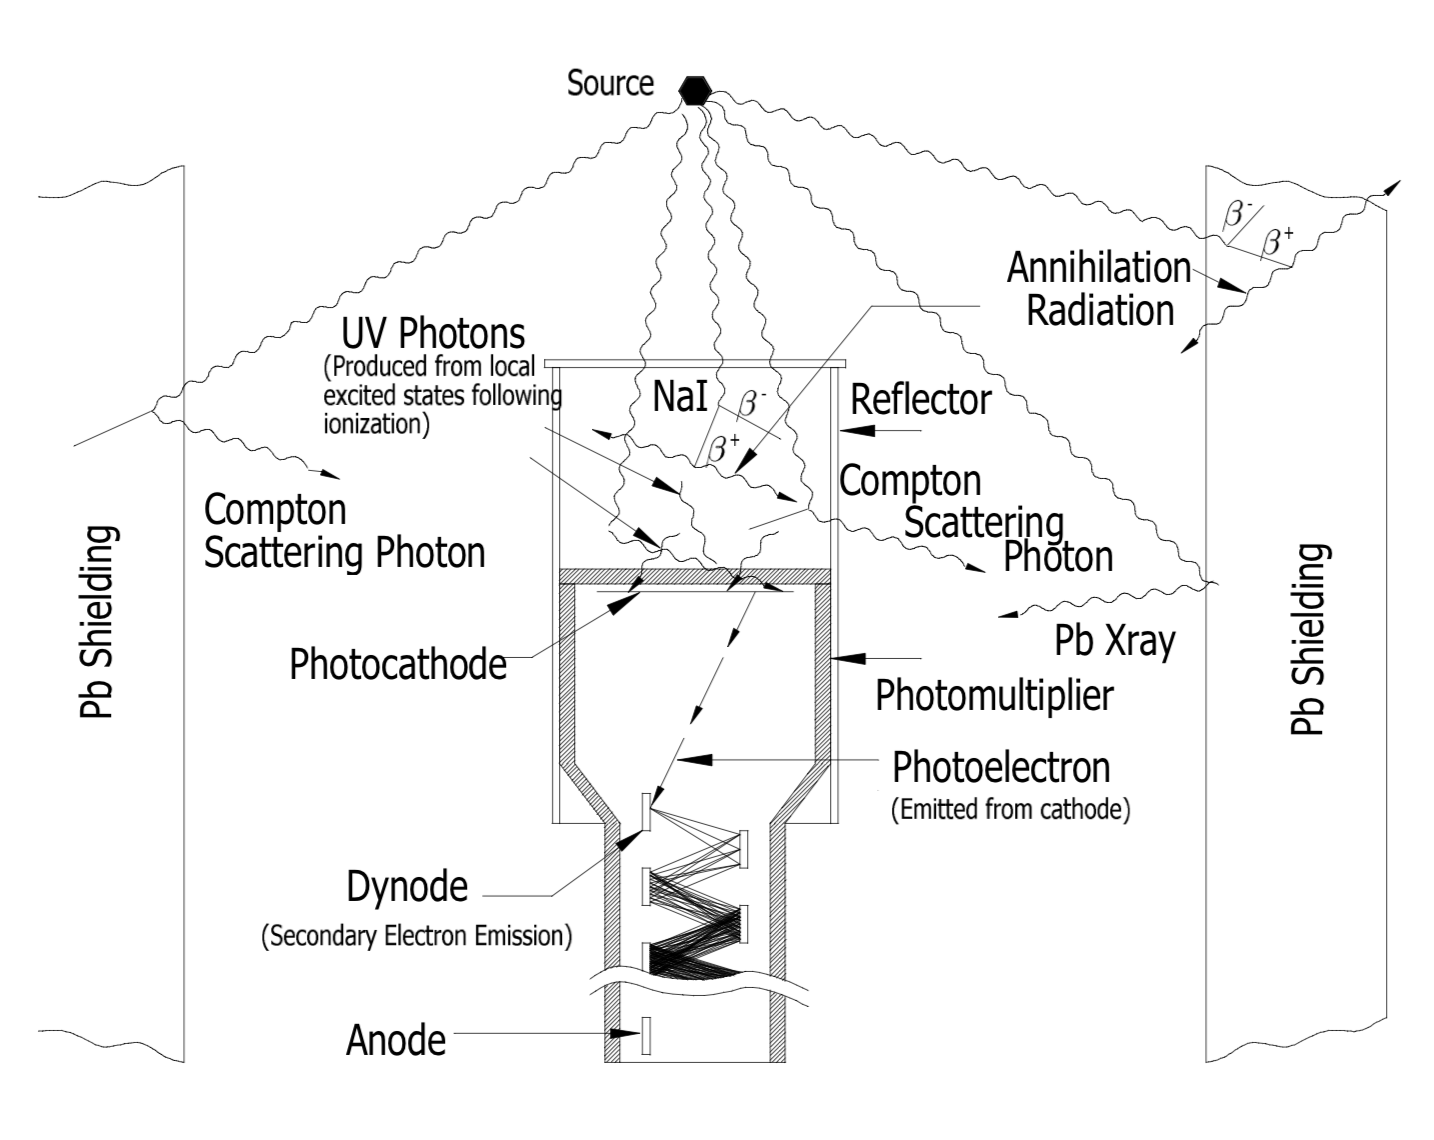
\includegraphics[width=1\linewidth]{lateximages/PMT.png}
\caption{\label{fig:PMT}  NaI scintillation crystal detector and photomultiplier tube. Gamma rays emitted from the source interact with the NaI scintillation crystal through the photoelectric effect and Compton scattering. The scintillation crystal then emits visible photons which hit the photocathode. The photocathode releases photoelectrons which strike dynodes that liberate more electrons. The multiplying of electrons is repeated at each dynode until it hits a collector that outputs a current that is proportional to the energy of the incoming gamma rays. (Source: Ref 2)}
\end{figure}

\subsection{Determining the Gain of the PMT}
The number of photoelectrons that are liberated in the PMT is a function of the high voltage that is placed across the tube. In order to properly calibrate the experiment and determine the gain of the PMT, it is therefore necessary to measure the gain of the PMT as a function of the high voltage that is placed across it. \newline
\indent Using the $\mathrm {  ^ { 137 }Cs }$ source as a marker, the high voltage across the PMT was varied and the corresponding photopeak bin number on the PHA from the source was recorded. Using the value of the external amplification and the bin number, we converted the bin number recorded to the output voltage of the PMT using the following equation:

\begin{equation}
V _ { o u t } = \frac { \text{Bin Number}\times \frac { 8 } { 1024 } V } { \text {External Amplification} }
 \label{eq:six}
\end{equation}

\noindent where the $\frac { 8 } { 1024 }$ comes from the PHA reading up to 8 volts which are split into 1024 bins. By plotting the PMT output voltage vs the high voltage placed across it, and then performing a least squares fit, the gain of the PMT was determined to have the functional relationship of:

\begin{equation}
V _ { o u t } = (9.4\times10^{-26})(\text{High Voltage})^{8.414}
 \label{eq:seven}
\end{equation}

A plot of the PMT output voltage vs the high voltage can be seen in Fig.~\ref{fig:gain}. Note, the fit only includes values up to 560V. At higher high voltage values, the PMT output seemed to be leveling off. This was probably due to the high value of the external amplification that we were using which clipped the voltage pulse received at the input of the pulse height analyzer. Another reason may be due to the limitations on how many electrons can be liberated from the dynodes as the high voltage placed across the PMT determines the voltage placed across the dynodes in the PMT. The fit was determined to have a reduced chi-squared value of 0.004.

\begin{figure}[H]
\includegraphics[width=1\linewidth]{lateximages/gain.png} 
\caption{\label{fig:gain} Gain of the PMT as a function of the high voltage placed across it. A least squares fit was formed to find the power law dependence of the PMT output voltage vs high voltage. The fit had a reduced chi-squared value of 0.004.}
\end{figure}

The power law dependence of the PMT can be understood by referring back to Fig.~\ref{fig:PMT}. Because the kinetic energy of the liberated electrons in the PMT is dependent how on much high voltage is placed on the dynodes, the higher the kinetic energy of the liberated electrons striking a dynode, the more electrons the dynodes can release. As the high voltage across the PMT increases, more electrons are released exponentially through multiple dynodes and contributes to a higher PMT output voltage.


\subsection{Determining the Linearity of the External Amplifier}
While the gain of the PMT is important, the linearity of the external amplifier must also be determined to properly calibrate the gamma ray experiment. The linearity of the amplifier was tested using a SRS DG645 Digital Delay Pulse Generator and a dB attenuator. \newline
\indent The pulse generator's output was connected to the attenuator whose output was then connected to the external amplifier. The output of the external amplifier was then connected to the PHA. \newline
\indent By using again the $\mathrm {  ^ { 137 }Cs }$ source as a marker, we measured the output voltage/peak channel of the photopeak as the amplitude of the input pulse varied for three different gain settings. Using the fine and coarse gain adjustments on the external amplifier, we plotted the output peak channel voltages vs input pulse amplitude for external amplifications of 12x, 24x, and 48x with a 10 dB attenuation in Fig.~\ref{fig:linearity}. A least squares fit was performed for each gain setting.

\begin{figure}[H]
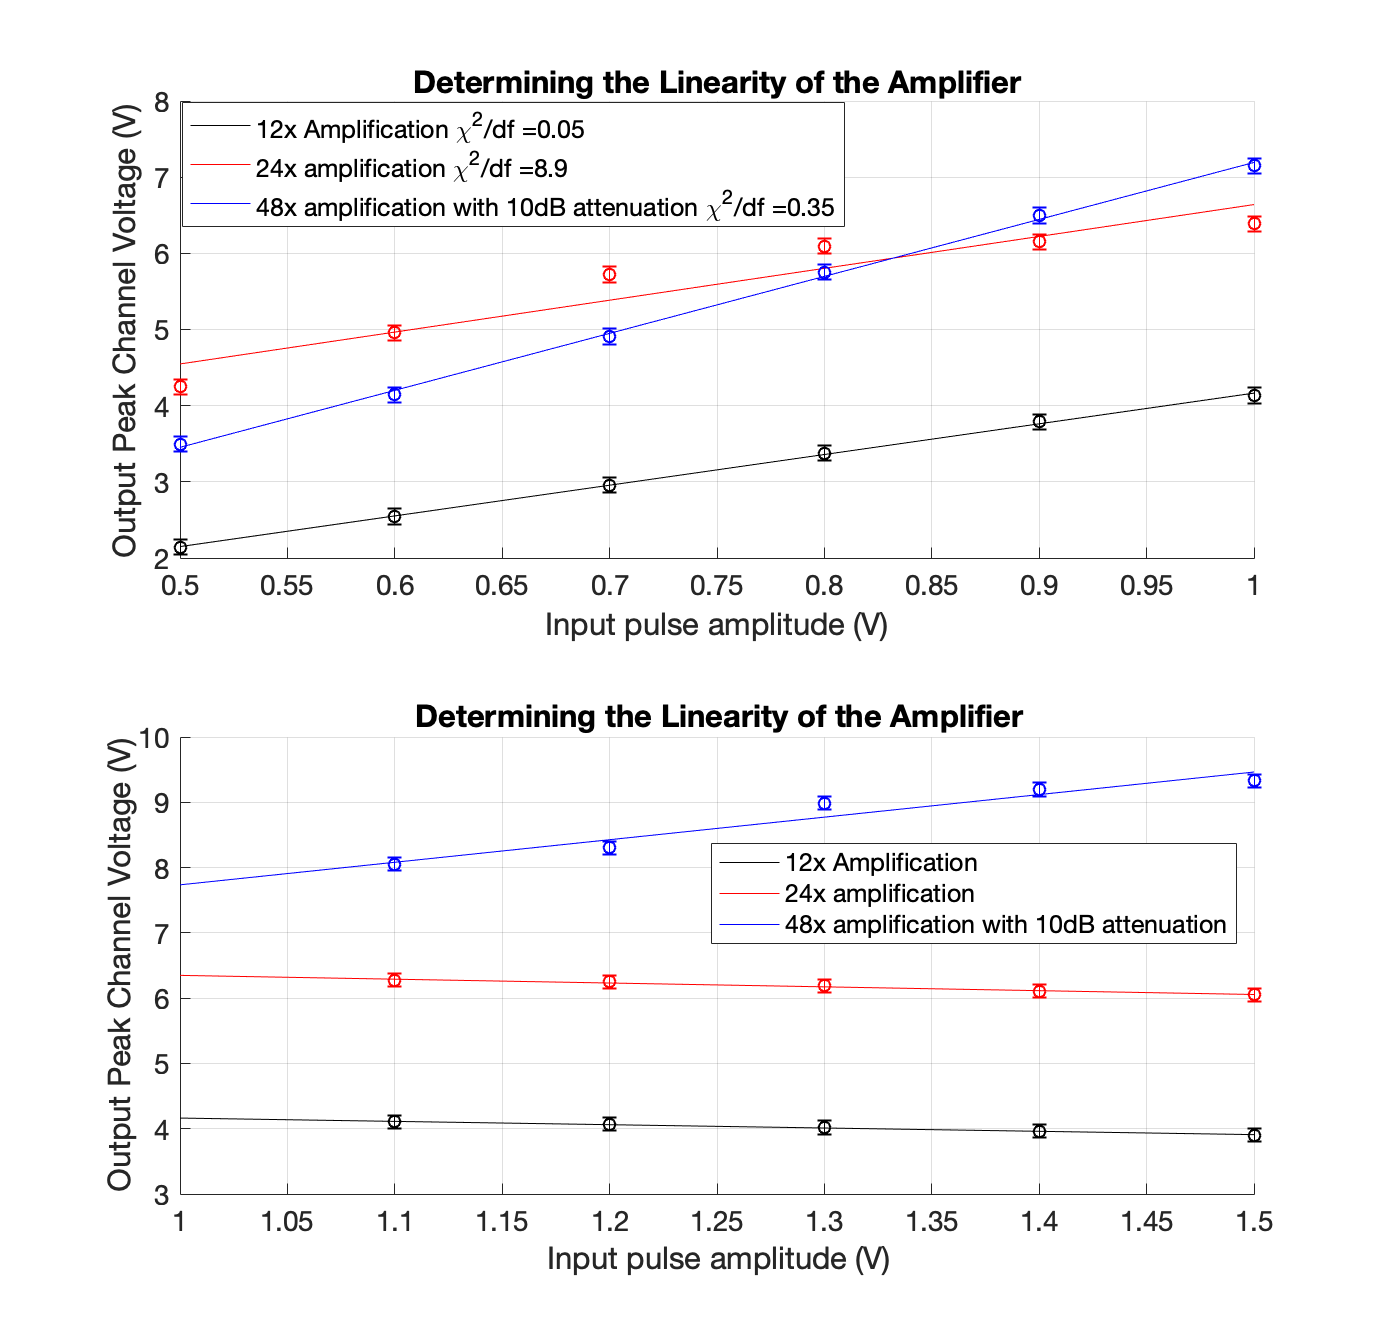
\includegraphics[width=1.1\linewidth]{lateximages/linearity.png} 
\caption{\label{fig:linearity} Determining the linearity of the external amplifier. The first graph shows the output peak channel voltages vs input pulse amplitudes from 0.5V to 1V. The second graph shows the output peak channel voltages vs input pulse amplitudes from 1V to 1.5V. At all amplifications tested, the amplifier was functioning linearly for input pulses of 0.5V to 1V. As the input pulse varied from 1V to 1.5V, however, we can see the clipping of the waveform by the external amplifier at amplifications of 12x and 24x. Note the error bars in each graph are small to the eye.}
\end{figure}

From the first graph of Fig.~\ref{fig:linearity}, we can see that at all three amplifications (12x, 24x, and 48x with a 10dB attenuation) that the graph stays increasingly linear with reduced chi-squared values of 0.05, 8.9, and 0.35, respectively for input pulses between 0.5V to 1V. The second graph in Fig.~\ref{fig:linearity}, however, shows that the output voltages are actually decreasing for 12x and 24x amplification with increasing input pulse amplitudes from 1V to 1.5V. We note that adding increased attenuation and/or decreasing the value of our external amplification fixes this problem at higher input pulse amplitudes. For this reason, the external amplifier was probably clipping the top of our input pulse leading to a lower output than expected in the second graph of Fig.~\ref{fig:linearity}. \newline
\indent In addition, the capabilities of the PHA were also analyzed by determining the relationship between the counts recorded by the PHA vs the rate of the pulse generator. At each repetition rate, the number of photopeak counts were recorded for a duration of 140 seconds. A linear fit was performed using the equation 

\begin{equation}
\text{Expected Counts}=\text{Repetition rate}\times \text{duration}
 \label{eq:eight}
\end{equation}

Fig.~\ref{fig:repetitionrate} is a plot of the counts recorded by the PHA versus repetition rate.

\begin{figure}[H]
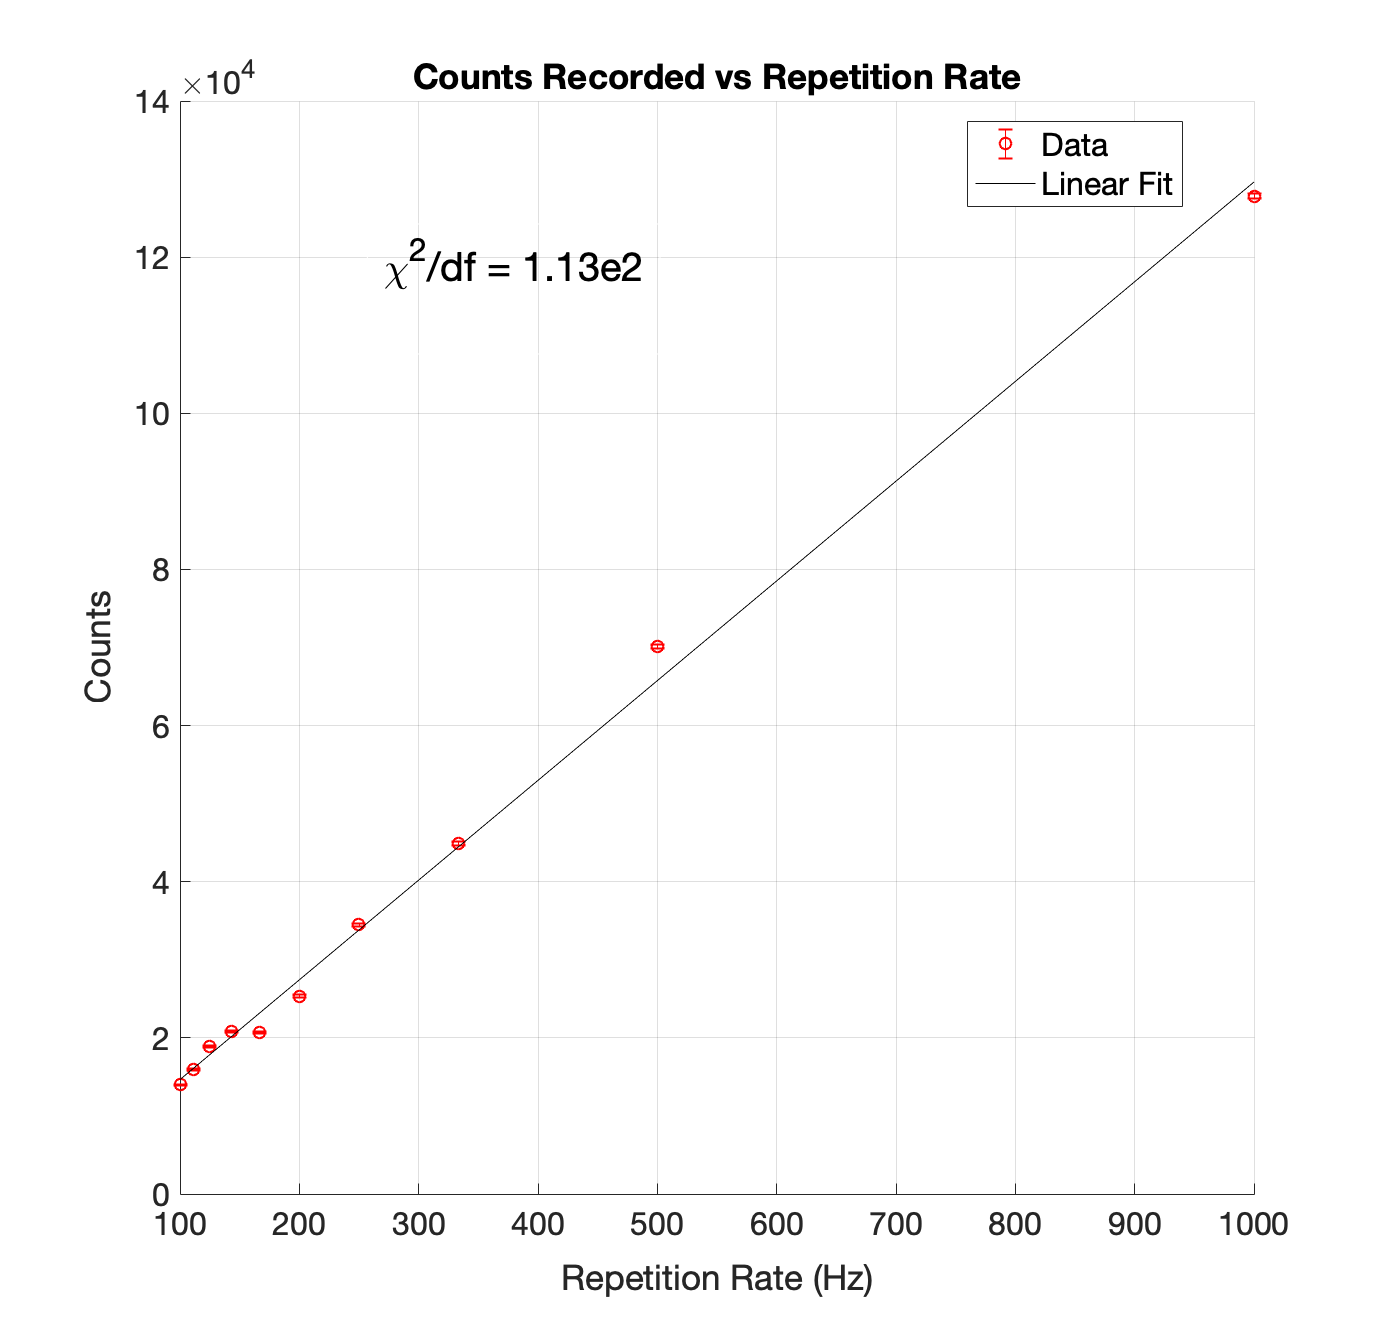
\includegraphics[width=1\linewidth]{lateximages/repetitionrate.png} 
\caption{\label{fig:repetitionrate} Photopeak counts vs pulse generator repetition rate. The counts recorded by the PHA increase as expected with increasing repetition rate. The reduced chi-squared goodness of fit value was $1.13\times10^2$. Note the error bars which are $\sqrt{\text{Counts}}$ are too small to see. }
\end{figure}

From Fig.~\ref{fig:repetitionrate}, we can see that the counts under the peak increase as expected with the linear fit, whose reduced chi-squared value was $1.13\times10^2$.



\section{Results and Analysis}
Once the capabilities of the PMT, PHA, and external amplifier was determined, data involving the sources can now be taken. A full block diagram of the experimental setup for collecting the spectra of the sources is shown in Fig.~\ref{fig:block}. \newline

\begin{figure}[H]
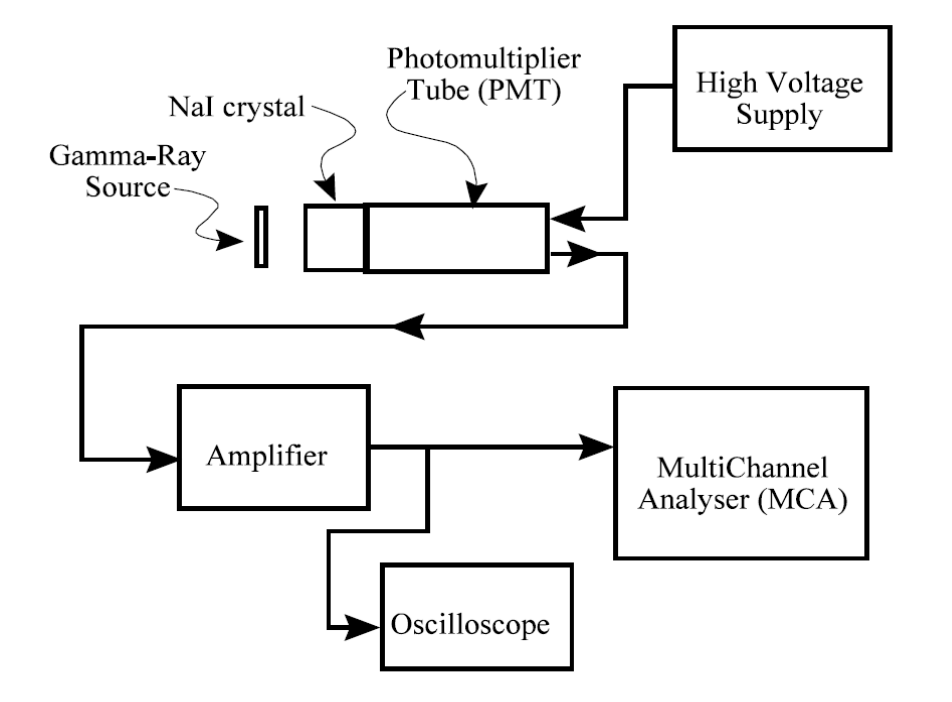
\includegraphics[width=1\linewidth]{lateximages/block.png} 
\caption{\label{fig:block} Block Diagram of Gamma Ray Spectroscopy setup. Note the MCA is the PHA. (Source: Ref. 4)}
\end{figure}

\indent For the rest of the following experiments and results, the PMT high voltage was kept at 560V and the external amplification was kept at 24x to maintain linearity.

\subsection{Spectral Analysis of $^ {\textbf{60}}\textbf{Co}$, $^ {\textbf{137}}\textbf{Cs}$, $^ {\textbf{22}}\textbf{Na}$, and $^ {\textbf{54}}\textbf{Mn}$}
The spectrum of each source was recorded by the PHA for a duration of 300 seconds with the sources a distance of 20 cm away from the detector. Since the PHA does not record energy values but bin numbers, the energy spectrums were calibrated using the known values of the photopeaks of each source. After collecting the four spectra, a linear fit was obtained by a least squares method using the following equation:

\begin{equation}
\text{Energy}=\text{Bin Number}\times m+b
 \label{eq:nine}
\end{equation}

\noindent where m and b are unknown constants that were determined after fitting this line to known photopeak energy values versus photopeak bin number recorded. The fit was determined to have a reduced chi-squared value of 36.17. The energy spectrum of the four sources is shown in Fig.~\ref{fig:4spectra}. 



\begin{figure*}
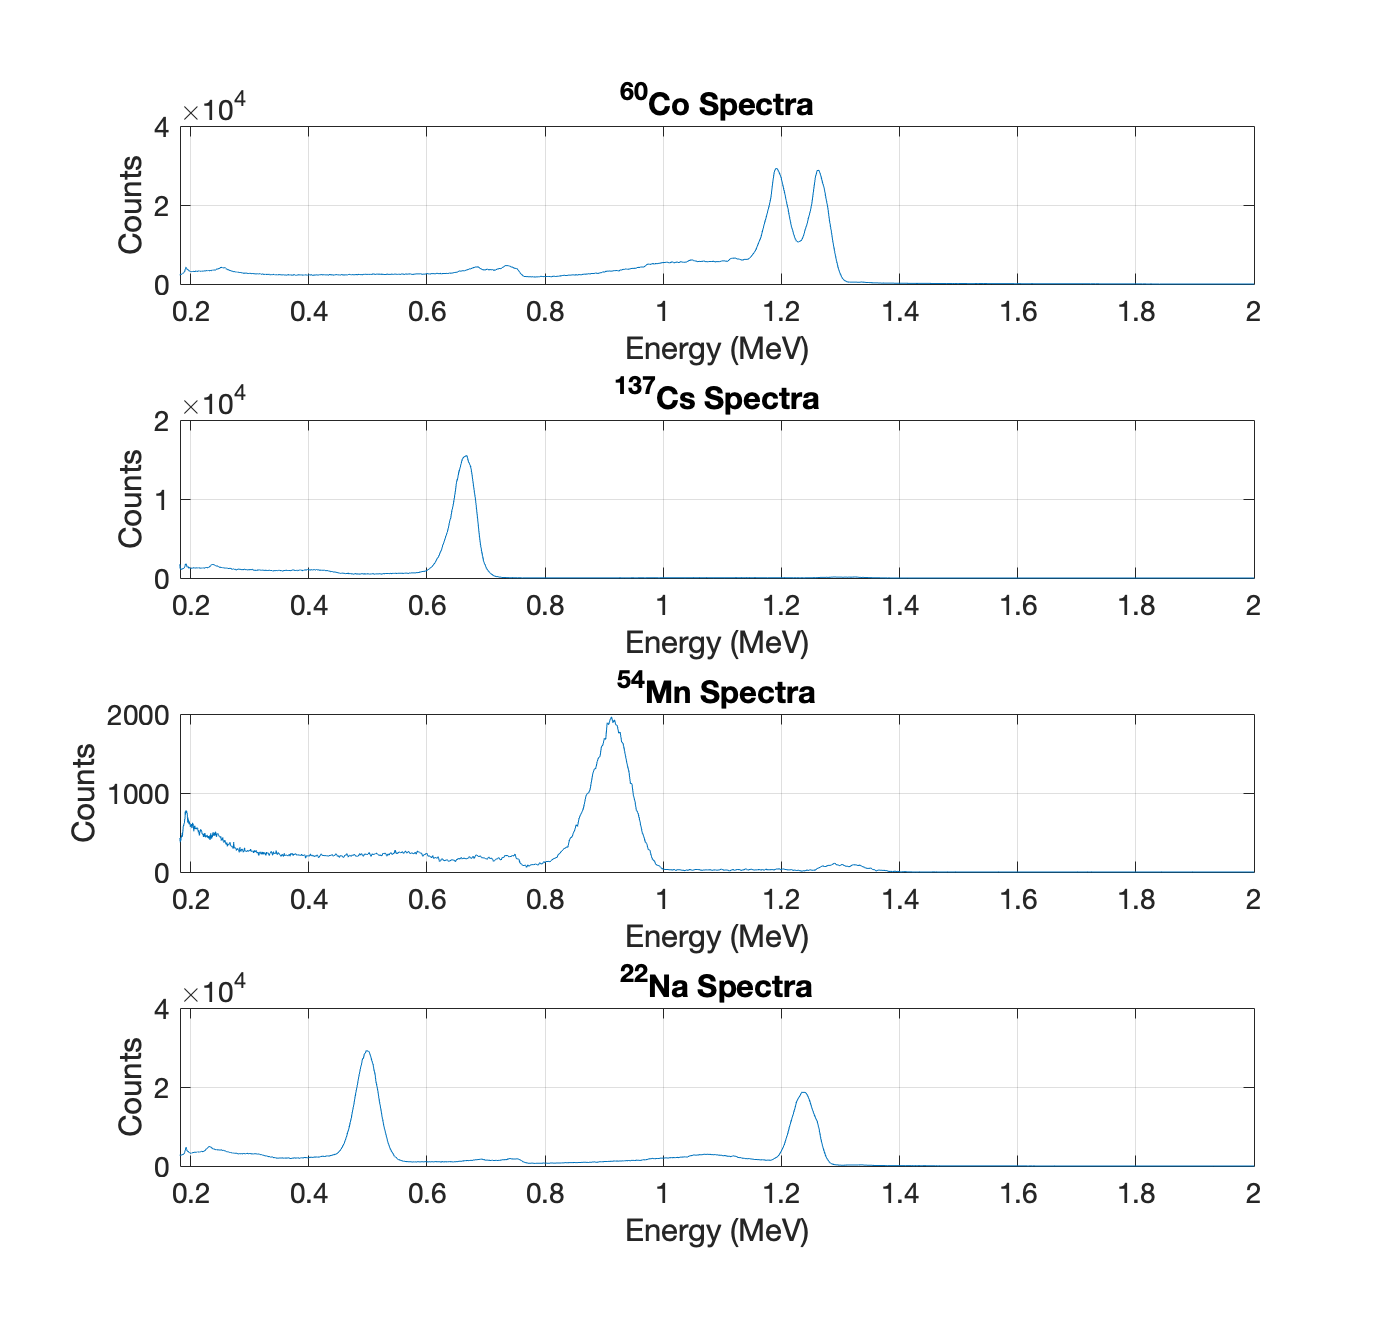
\includegraphics[width=0.9\linewidth]{lateximages/4spectra.png} 
\caption{\label{fig:4spectra} Energy Spectrum of $\mathrm { ^ { 60 }Co}  $, $\mathrm {  ^ { 137 }Cs }$, $\mathrm { ^ { 22 }Na }$, and $\mathrm { ^ { 54 }Mn } $. The energy axis was calibrated using known photopeak energy values by Eq.~(\ref{eq:nine}). The photopeaks, backscatter peaks, and Compton edges can be seen in each spectrum. }
\end{figure*}

\indent In the following subsections, we will be analyzing the spectrum of each source to determine the values of the photopeak, backscatter peak, and Compton edge energies. By calibrating the energy values through the linear fit described previously, these energies can be obtained. \newline
\indent The uncertainty in these measurements were obtained through a Gaussian fit on the relevant peaks and extracting its standard deviation $\sigma_E$ value, which is the uncertainty in the measured energy values. Once the uncertainty $\sigma_E$ is obtained for a photopeak, the full width at half maximum (FWHM) of the photopeak can be calculated using the relationship between the standard deviation $\sigma_E$ and FWHM for a Gaussian fit, which is 

\begin{equation}
\text{FWHM}=2.35 \times \sigma_E
 \label{eq:ten}
\end{equation}

The resolution at the energy of each photopeak can then be calculated as 

\begin{equation}
\text{Resolution}=\frac{\text{FWHM}}{E_{peak}}
 \label{eq:eleven}
\end{equation}

where $E_{peak}$ is the photopeak energy. \newline
\indent In the following subsections 1,2,3, and 4, the actual (theoretical) and measured energy values for each radioactive source are presented, along with their uncertainties, FWHM, and energy resolution that were calculated as just discussed. Note that the theoretical Compton edge energies and backscatter peak energies were obtained by Eq.~(\ref{eq:four}) and Eq.~(\ref{eq:five}), respectively. Referring to Fig.~\ref{fig:4spectra} will be helpful in illustrating the measured values in the following subsections.



\subsubsection{$\bf{ ^ { 137 }Cs }$ Spectra }
The $^ { 137 }$Cs  spectra was found to have a photopeak at 0.668 MeV $\pm$ 0.018 MeV as compared to the actual value of 0.661 MeV. The Compton edge energy was found to be 0.4296 MeV $\pm$ 0.053 MeV and the backscatter peak was measured to have a value of 0.191 MeV $\pm$ 0.013 MeV. Table~\ref{tab:table1} demonstrates a record of these results and their uncertainties, along with the FWHM and resolution of the photopeak.

\begin{table}[H]
\caption{\label{tab:table1}$\mathrm {  ^ { 137 }Cs }$ spectra }
\begin{ruledtabular}
\begin{tabular}{cccc}
&Photopeak&Compton Edge&Backscatter\\
\hline
Theoretical(MeV)&0.661&0.477 &0.181 \\
\hline
Measured(MeV)&0.668$\pm\sigma_E$&0.4296$\pm\sigma_E$&0.191$\pm\sigma_E$\\
\hline
$\sigma_E$ &0.018 & 0.053 & 0.013\\
\hline
FWHM &0.042 &  & \\
\hline
Resolution &6.35$\%$ &  & \\
\end{tabular}
\end{ruledtabular}
\end{table}

These measured energies were all found to be within the uncertainty of their actual values, indicating that the energy calibration fit was quite good for the $^ { 137 }$Cs source.

\subsubsection{$\bf{ ^ { 60 }Co }$ Spectra }
The $^ {60}$Co  spectra was found to have two photopeaks at 1.190 MeV $\pm$ 0.015 MeV and 1.264 MeV $\pm$ 0.011 MeV as compared to the actual values of 1.173 MeV and 1.332 MeV, respectively. The Compton edge energies were found to be 1.045 MeV $\pm$ 0.047 MeV and 1.12 MeV $\pm$ 0.013 MeV, respectively, and the backscatter peaks were measured to have a value of 0.192 MeV $\pm$ 0.023 MeV and 0.253 MeV $\pm$ 0.017 MeV, respectively. Table~\ref{tab:table2} demonstrates a record of these results and their uncertainties, along with the FWHM and resolution of the photopeaks.


\begin{table}[H]
\caption{\label{tab:table2}$\mathrm { ^ { 60 }Co}$ spectra }
\begin{ruledtabular}
\begin{tabular}{cccc}
&Photopeaks&Compton Edges&Backscatter\\
\hline
Theoretical(MeV)&1.173&0.963 &0.206\\
&1.332&1.11 &0.2105\\
\hline
Measured(MeV)&$1.190\pm\sigma_E$&$1.045\pm\sigma_E$&$0.192\pm\sigma_E$\\
&$1.2636\pm\sigma_E$&$1.12\pm\sigma_E$&$0.253\pm\sigma_E$\\
\hline
$\sigma_E$ &0.015& 0.047&0.023 \\
 &0.011&  0.013 & 0.017\\
 \hline
FWHM &0.035& & \\
&0.027&  & \\
\hline
Resolution &$3.02\%$ &  & \\
 &$2\%$ &  & \\
\end{tabular}
\end{ruledtabular}
\end{table}

Although the measured energy values were not as close to the actual values as compared to the $^ { 137 }$Cs source, the values are still fairly close. The measured photopeak values deviates at a maximum of 9$\%$ from its actual value, the Compton edge energies deviate at a maximum of approximately 8$\%$ from its actual value, and the backscatter peaks deviate at a maximum of approximately 18$\%$ from its actual value. This is expected as only the photopeaks were used to calibrate the energy spectrum and the nonlinearity in the amplifier also could have played a part in these relatively small deviations.


\subsubsection{$\bf{ ^ { 22 }Na }$ Spectra }
The $^ {22}$Na  spectra was found to have two photopeaks at 0.501 MeV $\pm$ 0.023 MeV and 1.24 MeV $\pm$ 0.013 MeV as compared to the actual values of 0.511 MeV and 1.27 MeV, respectively. The Compton edge energies were found to be 0.315 MeV $\pm$ 0.037 MeV and 1.061 MeV $\pm$ 0.032 MeV, respectively, and the backscatter peaks were measured to have a value of 0.193 MeV $\pm$ 0.028 MeV and 0.223 MeV $\pm$ 0.026 MeV, respectively. Table~\ref{tab:table3} demonstrates a record of these results and their uncertainties, along with the FWHM and resolution of the photopeaks.

\begin{table}[H]
\caption{\label{tab:table3}$\mathrm { ^ { 22 }Na }$ spectra }
\begin{ruledtabular}
\begin{tabular}{cccc}
&Photopeaks&Compton Edges&Backscatter\\
\hline
Theoretical(MeV)&0.511&0.340&0.168\\
&1.27&1.06 &0.209\\
\hline
Measured(MeV)&$0.501\pm\sigma_E$&$0.315\pm\sigma_E$&$0.193\pm\sigma_E$\\
&$1.24\pm\sigma_E$&$1.061\pm\sigma_E$&$0.223\pm\sigma_E$\\
\hline
$\sigma_E$ &0.023& 0.037 &0.028 \\
 &0.013& 0.032&0.026 \\
 \hline
FWHM &0.054&  & \\
&0.03&  & \\
\hline
Resolution &$10.78\%$ &  & \\
 &$2.3\%$ &  & \\
\end{tabular}
\end{ruledtabular}
\end{table}

The measured photopeak values were found to be fairly close to the actual photopeak values, which is expected as they were used to calibrate the spectrum. The measured Compton edge energies were also fairly close to their actual values, lying within one uncertainty of the actual values. The backscatter peaks deviated slightly more, but with both lying within two uncertainties of their actual values. The slightly more deviation by the backscatter peaks is expected as only the photopeaks were used to calibrate the spectrum, with the backscatter peak energies lying well below the energies used to calibrate the spectrum.

\subsubsection{$\bf{ ^ { 54 }Mn }$ Spectra }
The $^ { 54 }$Mn  spectra was found to have a photopeak at 0.912 MeV $\pm$ 0.027 MeV as compared to the actual value of 0.835 MeV. The Compton edge energy was found to be 0.7491 MeV $\pm$ 0.067 MeV and the backscatter peak was measured to have a value of 0.191 MeV $\pm$ 0.038 MeV. Table~\ref{tab:table4} demonstrates a record of these results and their uncertainties, along with the FWHM and resolution of the photopeak.

\begin{table}[H]
\caption{\label{tab:table4}$\mathrm { ^ { 54 }Mn } $ spectra }
\begin{ruledtabular}
\begin{tabular}{cccc}
&Photopeak&Compton Edge&Backscatter\\
\hline
Theoretical(MeV)&0.835&0.639 &0.192 \\
\hline
Measured(MeV)&$0.912\pm\sigma_E$&$0.7491\pm\sigma_E$&$0.191\pm\sigma_E$\\
\hline
$\sigma_E$ &0.027&0.067 &0.038 \\
\hline
FWHM &0.063 &  & \\
\hline
Resolution &$7.5\%$ &  & \\
\end{tabular}
\end{ruledtabular}
\end{table}
The measured value of the photopeak deviates about 9$\%$ from the actual photopeak value, while the measured Compton edge energy is within two uncertainty of its actual value. The measured backscatter peak is nearly identical to its actual value. Again, deviations are expected as the experimental setup may not be functioning entirely linearly and our fit being not entirely perfect. In all, most of our measured values were quite close to the actual values for all sources, indicating that the equipment was functioning well for our purpose and that the energy calibration was adequate in describing the spectrum of the sources.

\subsection{ Inverse Square Law}
In contrast to other types of radiation like beta radiation, gamma rays have an intensity that is inversely proportional to the square of the distance from the source. Using the $^ { 137 }$Cs source as a marker, we collected its spectra for various distances (from 25cm to 75cm) from the detector with a duration of 300s for each distance.

\begin{figure}[H]
\centering
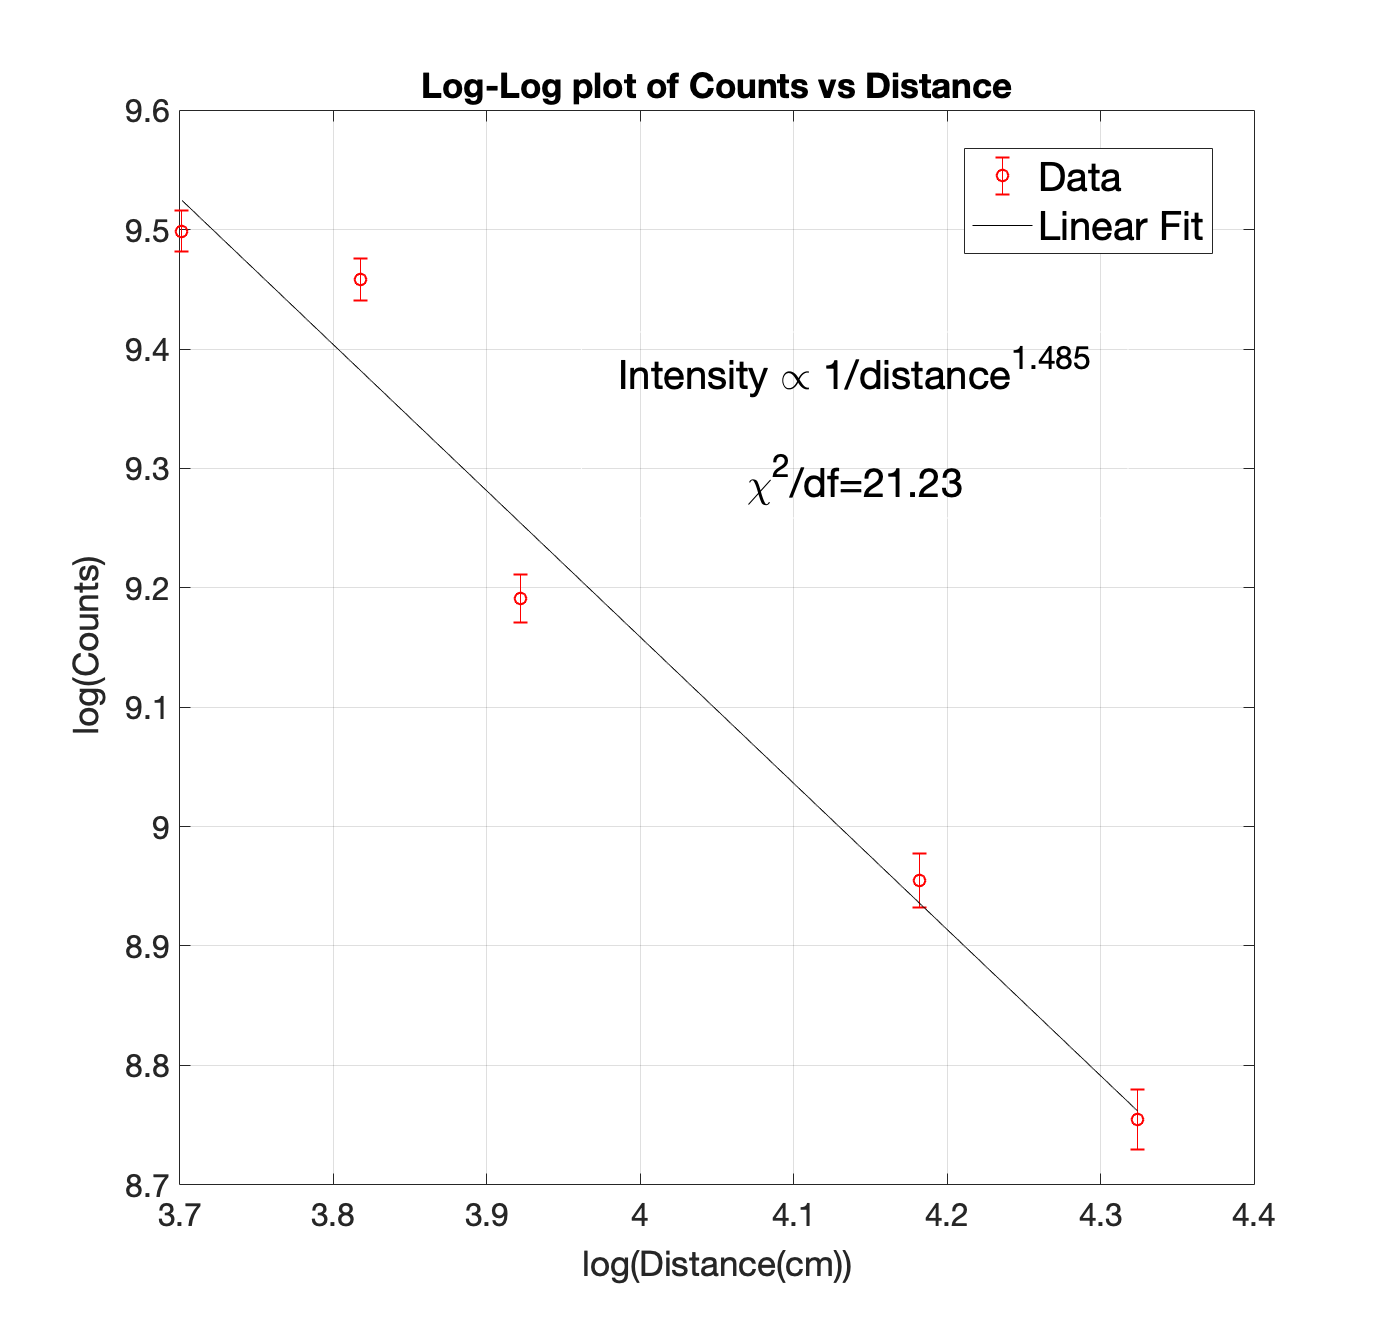
\includegraphics[width=0.95\linewidth]{lateximages/inversesquare.png} 
\caption{\label{fig:inversesquare}  Log-Log plot of photopeak counts vs source distance from detector}
\end{figure}

By recording the number of counts at the photopeak energy for each distance, a log-log plot of the Counts vs source distance from detector was obtained in Fig.~\ref{fig:inversesquare}. A linear fit on these log-log data points was performed, with reduced chi-squared value 21.23, and the gamma ray intensity was determined to have the relationship

\begin{equation}
\text{Counts}=\text{Intensity}\propto \frac{1}{\text{distance}^{1.485}}
 \label{eq:twelve}
\end{equation}

Although the value of 1.485 is not exactly 2, it is relatively close. Some possible reasons for the deviation are the limitations of the equipment on recording the counts and the errors in the distance measured. The finite size of the detector also plays a role in the deviations.


\subsection{Absolute Intensity of $\bf{ ^ { 137 }Cs }$ }
The absolute intensity of  $^ { 137 }$Cs can be computed by the equation

\begin{equation}
I_{measured}=I_{absolute}\times [n(E) \frac{\Delta \Omega}{4\pi}]
 \label{eq:thirteen}
\end{equation}

\noindent where n(E) is the intrinsic efficiency and $\Delta \Omega$ is the solid angle. Using the NaI crystal information for a distance of d=25cm and a gamma ray energy of 0.662 MeV, the quantity in brackets was given as 0.2$\%$. \newline
\indent The spectra of $^ { 137 }$Cs and also a background subtraction was taken (which turned out to be approximately 25 counts in 150 sec) for 150 sec, and $I_{measured}$ was $58\pm0.62$ counts/sec. Dividing by 0.2$\%$, we have that the absolute intensity of $^ { 137 }$Cs is 

\begin{equation}
I_{absolute}= 29,000\pm310 \text{ counts/sec}
 \label{eq:fourteen}
\end{equation}


\subsection{Mass Attenuation Coefficients of Cu, Al, and Pb}
Lastly, gamma ray intensities get attenuated when passing through materials (absorbers) of varying thickness. The intensity of the gamma rays following attenuation is given by

\begin{equation}
I= I_{0} e^{-\mu t}
 \label{eq:fifteen}
\end{equation}

\noindent where $\mu$ is the linear attenuation coefficient of the absorber, $I_{0}$ is the intensity of incident gamma ray before attenuation, and t is the thickness of the absorber. \newline
\indent Once the linear attenuation coefficient of the absorber is found, the mass attenuation coefficient of the material can be calculated using the equation 

\begin{equation}
\text{Mass Attenuation Coefficient}= \frac{\mu}{\rho}
 \label{eq:sixteen}
\end{equation}

\noindent where $\rho$ is the density of the absorber. \newline
\indent The mass attenuation coefficients of aluminum, copper, and lead, were measured using $^ {137 }$Cs and $^ { 22 }$Na sources. The setup of the this experiment is illustrated in Fig.~\ref{fig:MATexperiment}.

\begin{figure}[H]
\centering
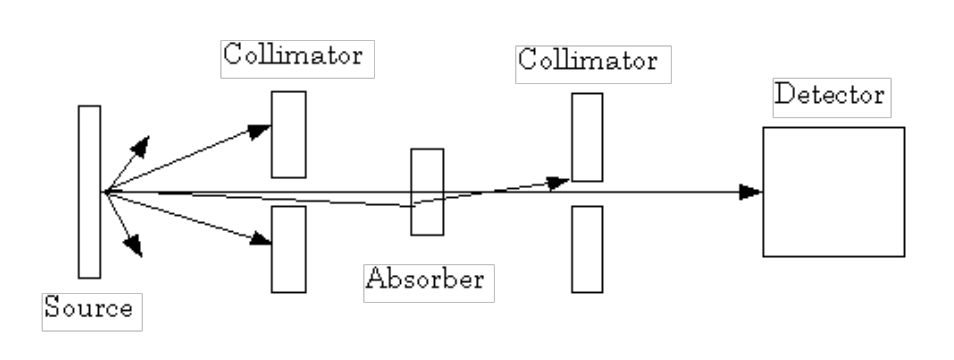
\includegraphics[width=1\linewidth]{lateximages/MATexperiment.png} 
\caption{\label{fig:MATexperiment} Experimental setup to measure the mass attenuation coefficients of Cu, Al, and Pb absorbers.}
\end{figure}

The sources were placed at 25cm from the detector, with collimators placed at 8cm and 24cm away from the detector. Absorbers of varying thickness were placed in between these collimators and the intensity was recorded for each source, along with intensities without any absorber, for a duration of 180 sec each. \newline
\indent Once the intensities as a function of varying absorber thickness was determined, the linear attenuation coefficient was determined by fitting a straight line to the equation 

\begin{equation}
ln(I)= -\mu t + ln(I_{0})
 \label{eq:seventeen}
\end{equation}

where the slope of the line, $\mu$, is the linear attenuation coefficient of the material. Fig.~\ref{fig:cs137attenuation} and Fig.~\ref{fig:na22attenuation} illustrates these results. \newline
\indent In Fig.~\ref{fig:cs137attenuation}, plots of the natural log of intensity vs absorber thickness for each absorber was plotted along with a straight line fit using Eq.~(\ref{eq:seventeen}) for the $^ {137 }$Cs source. The linear attenuation coefficients for Cu, Al, and Pb were found to be 0.057$\pm$0.0008 $\frac{1}{mm}$, 0.018$\pm$0.0014 $\frac{1}{mm}$, 0.131$\pm$0.0076 $\frac{1}{mm}$, respectively. The reduced chi-squared values of the fit were $9.5\times10^{-4}$, $6.8\times10^{-4}$, $0.06$, respectively. \newline 
\indent In Fig.~\ref{fig:na22attenuation}, plots of the natural log of intensity vs absorber thickness for each absorber was plotted along with a straight line fit using Eq.~(\ref{eq:seventeen}) for the $^ {22 }$Na source. The linear attenuation coefficients for Cu, Al, and Pb were found to be 0.064$\pm$0.0003 $\frac{1}{mm}$, 0.02$\pm$0.0007 $\frac{1}{mm}$, 0.199$\pm$0.067 $\frac{1}{mm}$, respectively. The reduced chi-squared values of the fit were $1.4\times10^{-4}$, $1.7\times10^{-3}$, $4.2$, respectively. \newline
\indent Once the linear attenuation coefficients were obtained, the mass attenuation coefficients of Cu, Al, and Pb were calculated using Eq.~(\ref{eq:sixteen}). A summary of these results can be found in Table~\ref{tab:table5} on the next page. Note the actual values of the mass attenuation coefficients in the table were obtained from reference 5. \newline
\indent From Table~\ref{tab:table5} , we can see that our measured values


\begin{figure}[H]
\centering
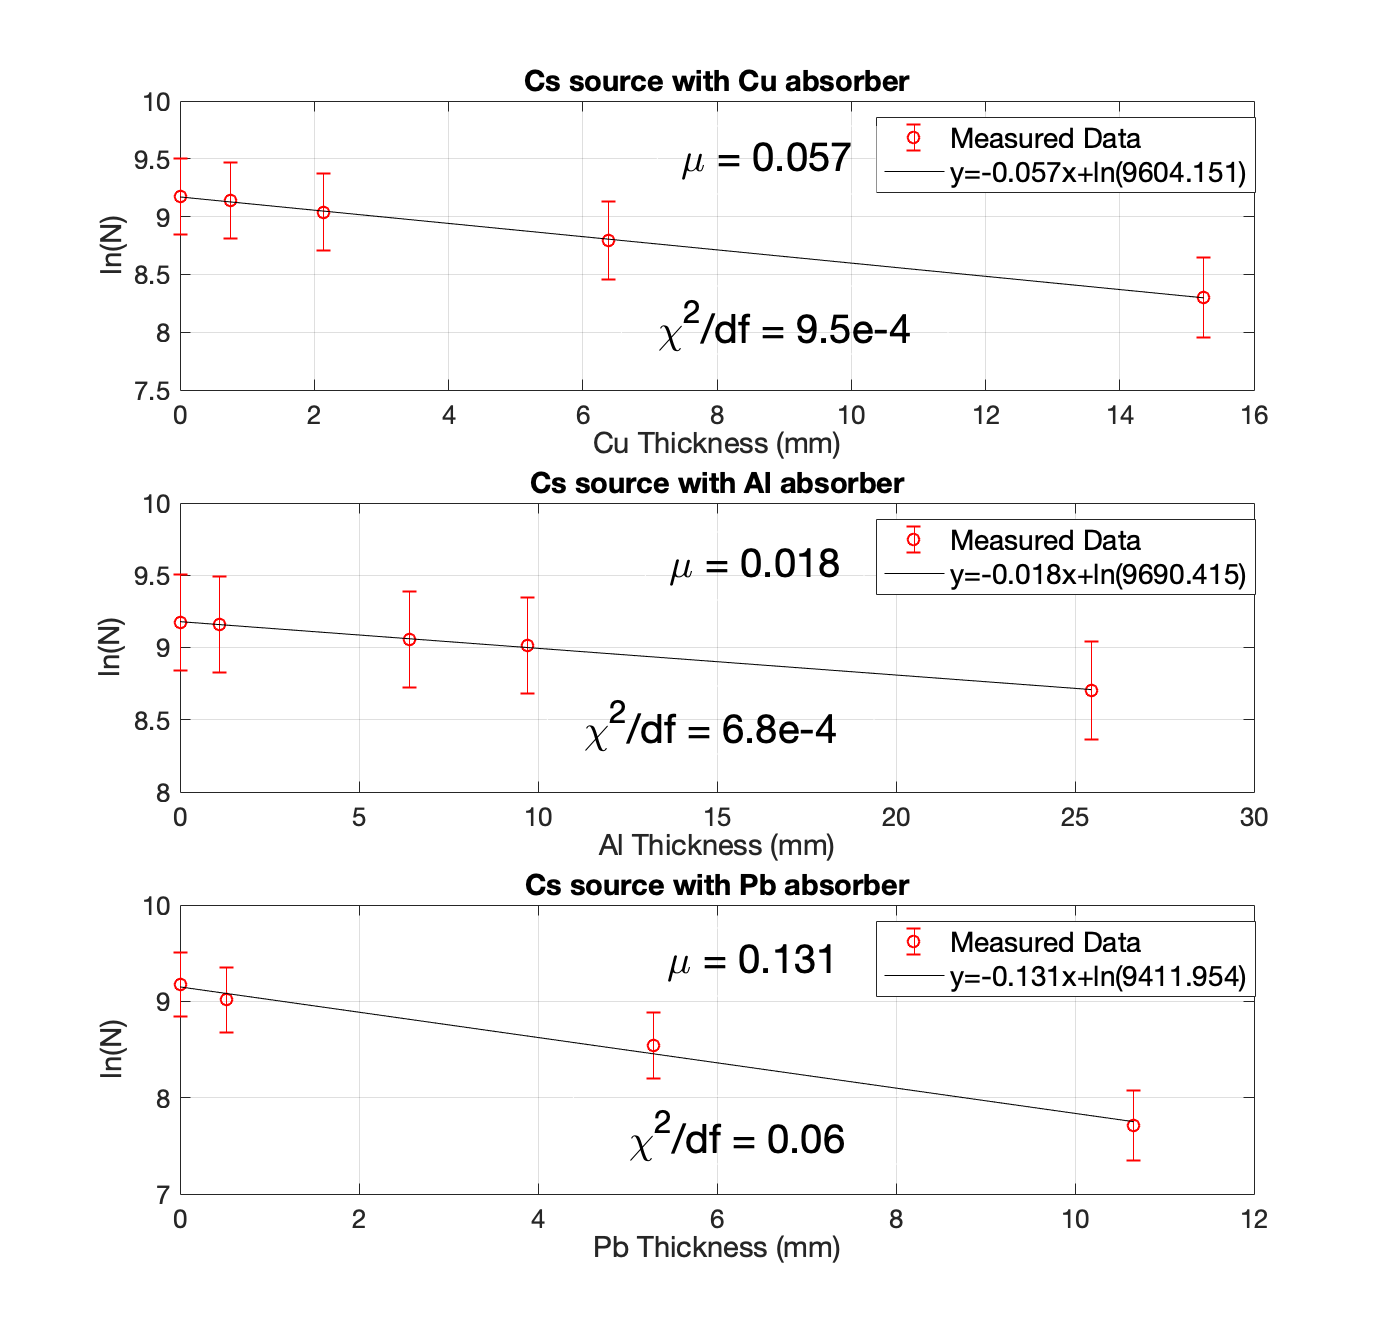
\includegraphics[width=1.05\linewidth]{lateximages/cs137atten.png} 
\caption{\label{fig:cs137attenuation} Semilog plot in the y-axis of Intensity vs absorber thickness for each absorber. The linear attenuation coefficients of Cu, Al, and Pb were obtained for a $^ {137 }$Cs source using a straight line fit according to Eq.~(\ref{eq:seventeen}). }
\end{figure}

\begin{figure}[H]
\centering
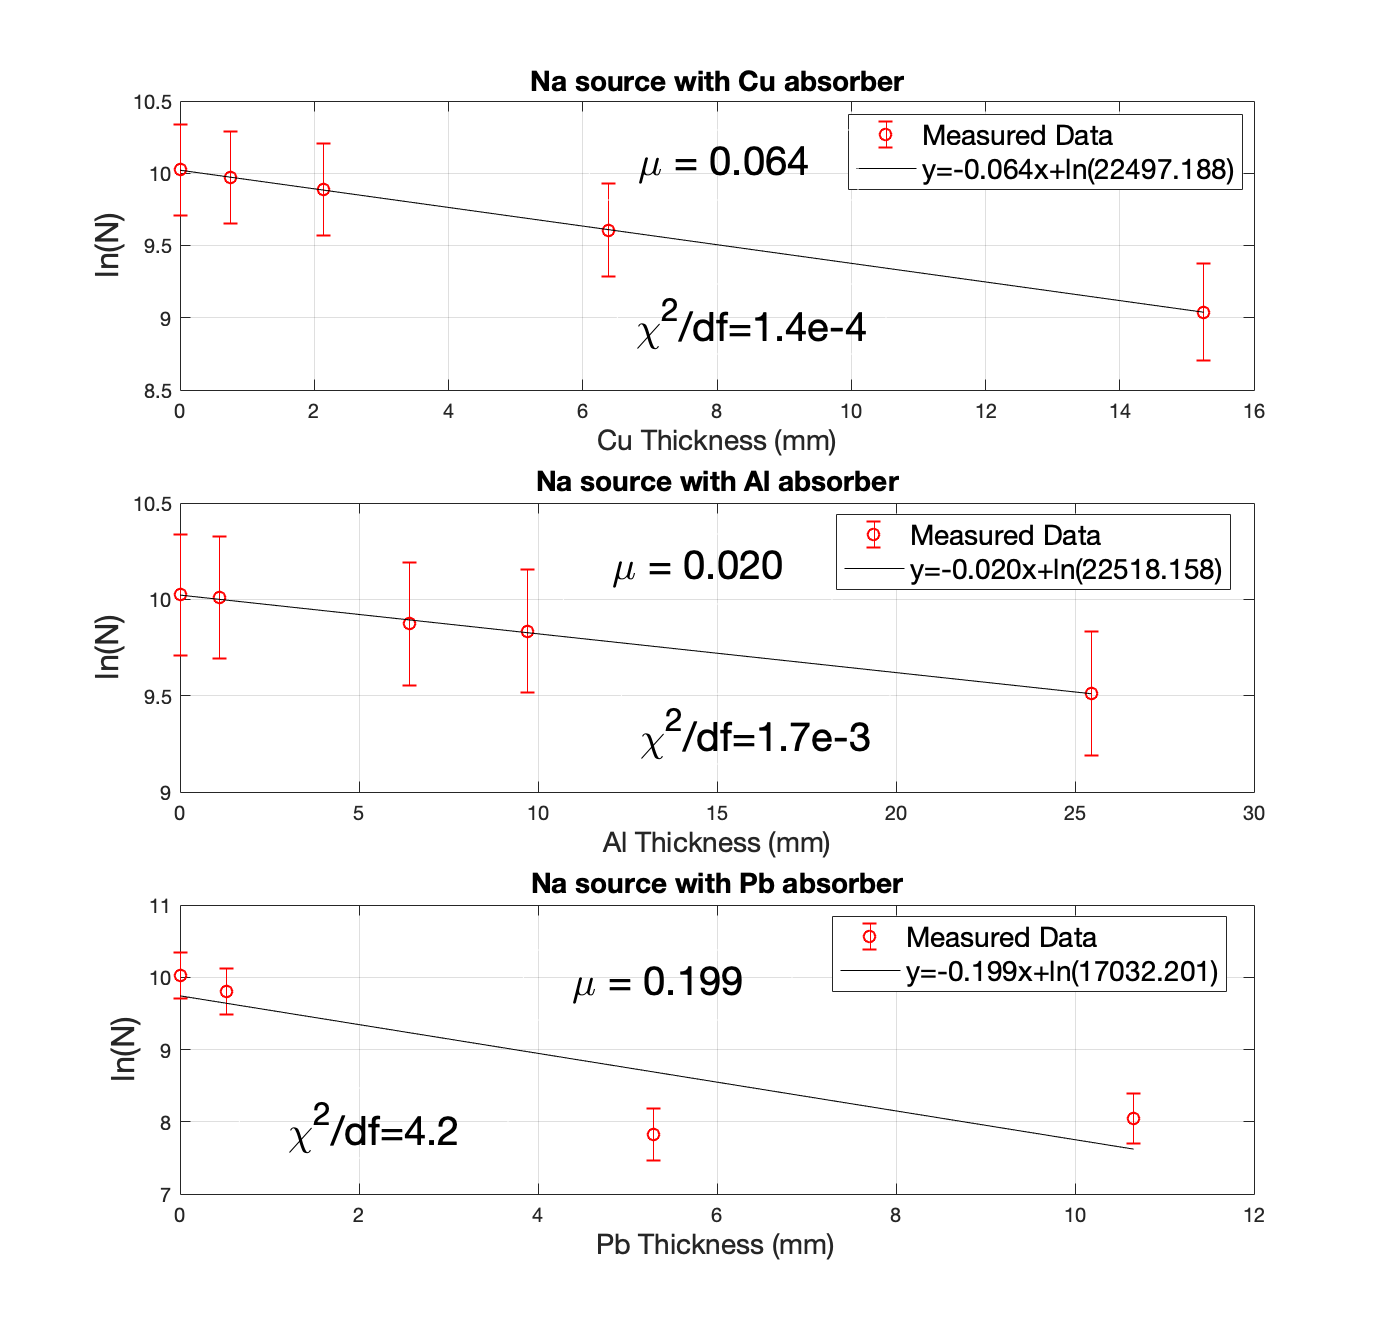
\includegraphics[width=1.05\linewidth]{lateximages/na22attenuation.png} 
\caption{\label{fig:na22attenuation} Semilog plot in the y-axis of Intensity vs absorber thickness for each absorber. The linear attenuation coefficients of Cu, Al, and Pb were obtained for a $^ {22 }$Na source using a straight line fit according to Eq.~(\ref{eq:seventeen}).}
\end{figure}

\begin{table*}
\caption{\label{tab:table5}Mass Attenuation Coefficients}
\begin{ruledtabular}
\begin{tabular}{cccccc}
Source&$\gamma(MeV)$&Absorber&$\mu (\frac{1}{mm})$&\text{Measured }$\frac{\mu}{\rho}(\frac{cm^2}{g})$&Actual $\frac{\mu}{\rho}(\frac{cm^2}{g})$\\
\hline
$\mathrm { ^ { 22 }Na }$&0.511& $\mathrm { Cu }$&$0.064\pm0.0003$&$0.071\pm0.00033$&0.117\\
\hline
$\mathrm { ^ { 22 }Na }$&0.511& $\mathrm { Al }$&$0.02\pm0.0007$&$0.074\pm0.0026$&0.111\\
\hline
$\mathrm { ^ { 22 }Na }$&0.511& $\mathrm { Pb }$&$0.199\pm0.067$&$0.175\pm0.059$&0.163\\
\hline
$\mathrm {  ^ { 137 }Cs }$&0.662& $\mathrm { Cu }$&$0.057\pm0.0008$&$0.064\pm0.0009$&0.089 \\
\hline
$\mathrm {  ^ { 137 }Cs }$&0.662& $\mathrm { Al }$&$0.018\pm0.0014$&$0.067\pm0.0051$&0.091 \\
\hline
$\mathrm {  ^ { 137 }Cs }$&0.662& $\mathrm { Pb }$&$0.131\pm0.0076$&$0.116\pm0.0067$&0.118\\
\end{tabular}
\end{ruledtabular}
\end{table*}

\noindent of the mass attenuation coefficient using the $^ {137 }$Cs source were 0.064$\pm$0.0009 $\frac{cm^2}{g}$, 0.067$\pm$0.0051 $\frac{cm^2}{g}$, 0.116$\pm$0.0067 $\frac{cm^2}{g}$ for Cu, Al, and Pb, respectively. While for the $^ {22 }$Na source, the mass attenuation coefficients were 0.071$\pm$0.00033 $\frac{cm^2}{g}$, 0.074$\pm$0.0026 $\frac{cm^2}{g}$, 0.175$\pm$0.059 $\frac{cm^2}{g}$ for Cu, Al, and Pb, respectively. \newline
\indent Compared to the actual values, the measured mass attenuation coefficients for lead are quite close to the actual values, whereas the coefficients for copper and aluminum deviate further, but well within an order of magnitude. What is surprising is that our measured values of the coefficients for aluminum were just slightly larger than copper. As expected, lead has the highest value of mass attenuation for both sources.

\section{Conclusion}
In conclusion, the spectra of $\mathrm { ^ { 60 }Co}  $, $\mathrm {  ^ { 137 }Cs }$, $\mathrm { ^ { 22 }Na }$, and $\mathrm { ^ { 54 }Mn } $ was obtained through gamma ray spectroscopy using a scintillation detector, a PMT, an external amplifier, and a pulse height analyzer. The gain of the PMT and the linearity of the external amplifier were also measured to calibrate the experiment. Through an energy calibration fit of the spectra, the photopeak, Compton edge, and backscatter peak energies of the four sources were measured, which were found to be within good agreement to their actual values. The intensity was found to have a dependence $\text{distance}^{-1.485}$, which deviates from the expected $\text{distance}^{-2}$ inverse square law. This deviation was attributed to systematic errors, measuring distance errors, and the finite size of the detector. The absolute intensity of $^ {137 }$Cs was also determined to be $29,000\pm310 \text{ counts/sec}$. Lastly, the mass attenuation coefficients of Cu,Al, and Pb were measured using the $^ {137 }$Cs and $^ {22 }$Na sources.



\begin{acknowledgments}
We would like to thank the Physics 111B staff for their patience and guidance during this experiment. Without you, we would still be trying to figure out how to setup the experiment. \newline

\end{acknowledgments}
 

\nocite{*}

 \begin{thebibliography}{1}
 

\bibitem{Knoll} G.F. Knoll, {\em "Radiation Detection and Measurement,"} John Wiley \& Sons, New York, 2010. \newline

\bibitem{florida}   {\em "Gamma Ray Spectroscopy - Experimental GRS," } University of Florida, Department of Physics,
PHY4803L - Advanced Physics Laboratory \newline

\bibitem{detectors} H.A. Smith Jr., M. Lucas, {\em "Gamma-Ray Detectors." } \newline

\bibitem{blockdiagram}  T. Tyson,  {\em "Gamma Spectroscopy," } University of California Davis, Department of Physics, Physics 122, 2019. \newline

\bibitem{attenuation}  S.Gjorgieva, L. Barandovski,  {\em "Measurement Of The Mass Attenuation Coefficient From 81
keV to 1333 keV For Elemental Materials Al, Cu And Pb," } AIP Conference Proceedings 1722, 180003, 2016. \newline




  \end{thebibliography}


\end{document}
%
% ****** End of file aipsamp.tex ******